\setAuthor{Richard Luhtaru}
\setRound{lahtine}
\setYear{2023}
\setNumber{G 2}
\setDifficulty{2}
\setTopic{TODO}

\prob{Kumerpeegel}
Joonisel (suurendatult lisalehel) on kujutatud ese AB ja kumerpeegel, mille keskpunkt on O ja fookus on F. Eeldame, et ese on sümmeetriateljest natuke nihkes, nii et see on punktist P nähtav nii otse kui kumerpeeglis. Mitu korda väiksem paistab ese AB punktist P kumerpeegli abil vaadelduna (võrreldes otse vaatamisega)? Lahendage ülesanne lisalehel.

\begin{figure}[h]
    \centering

    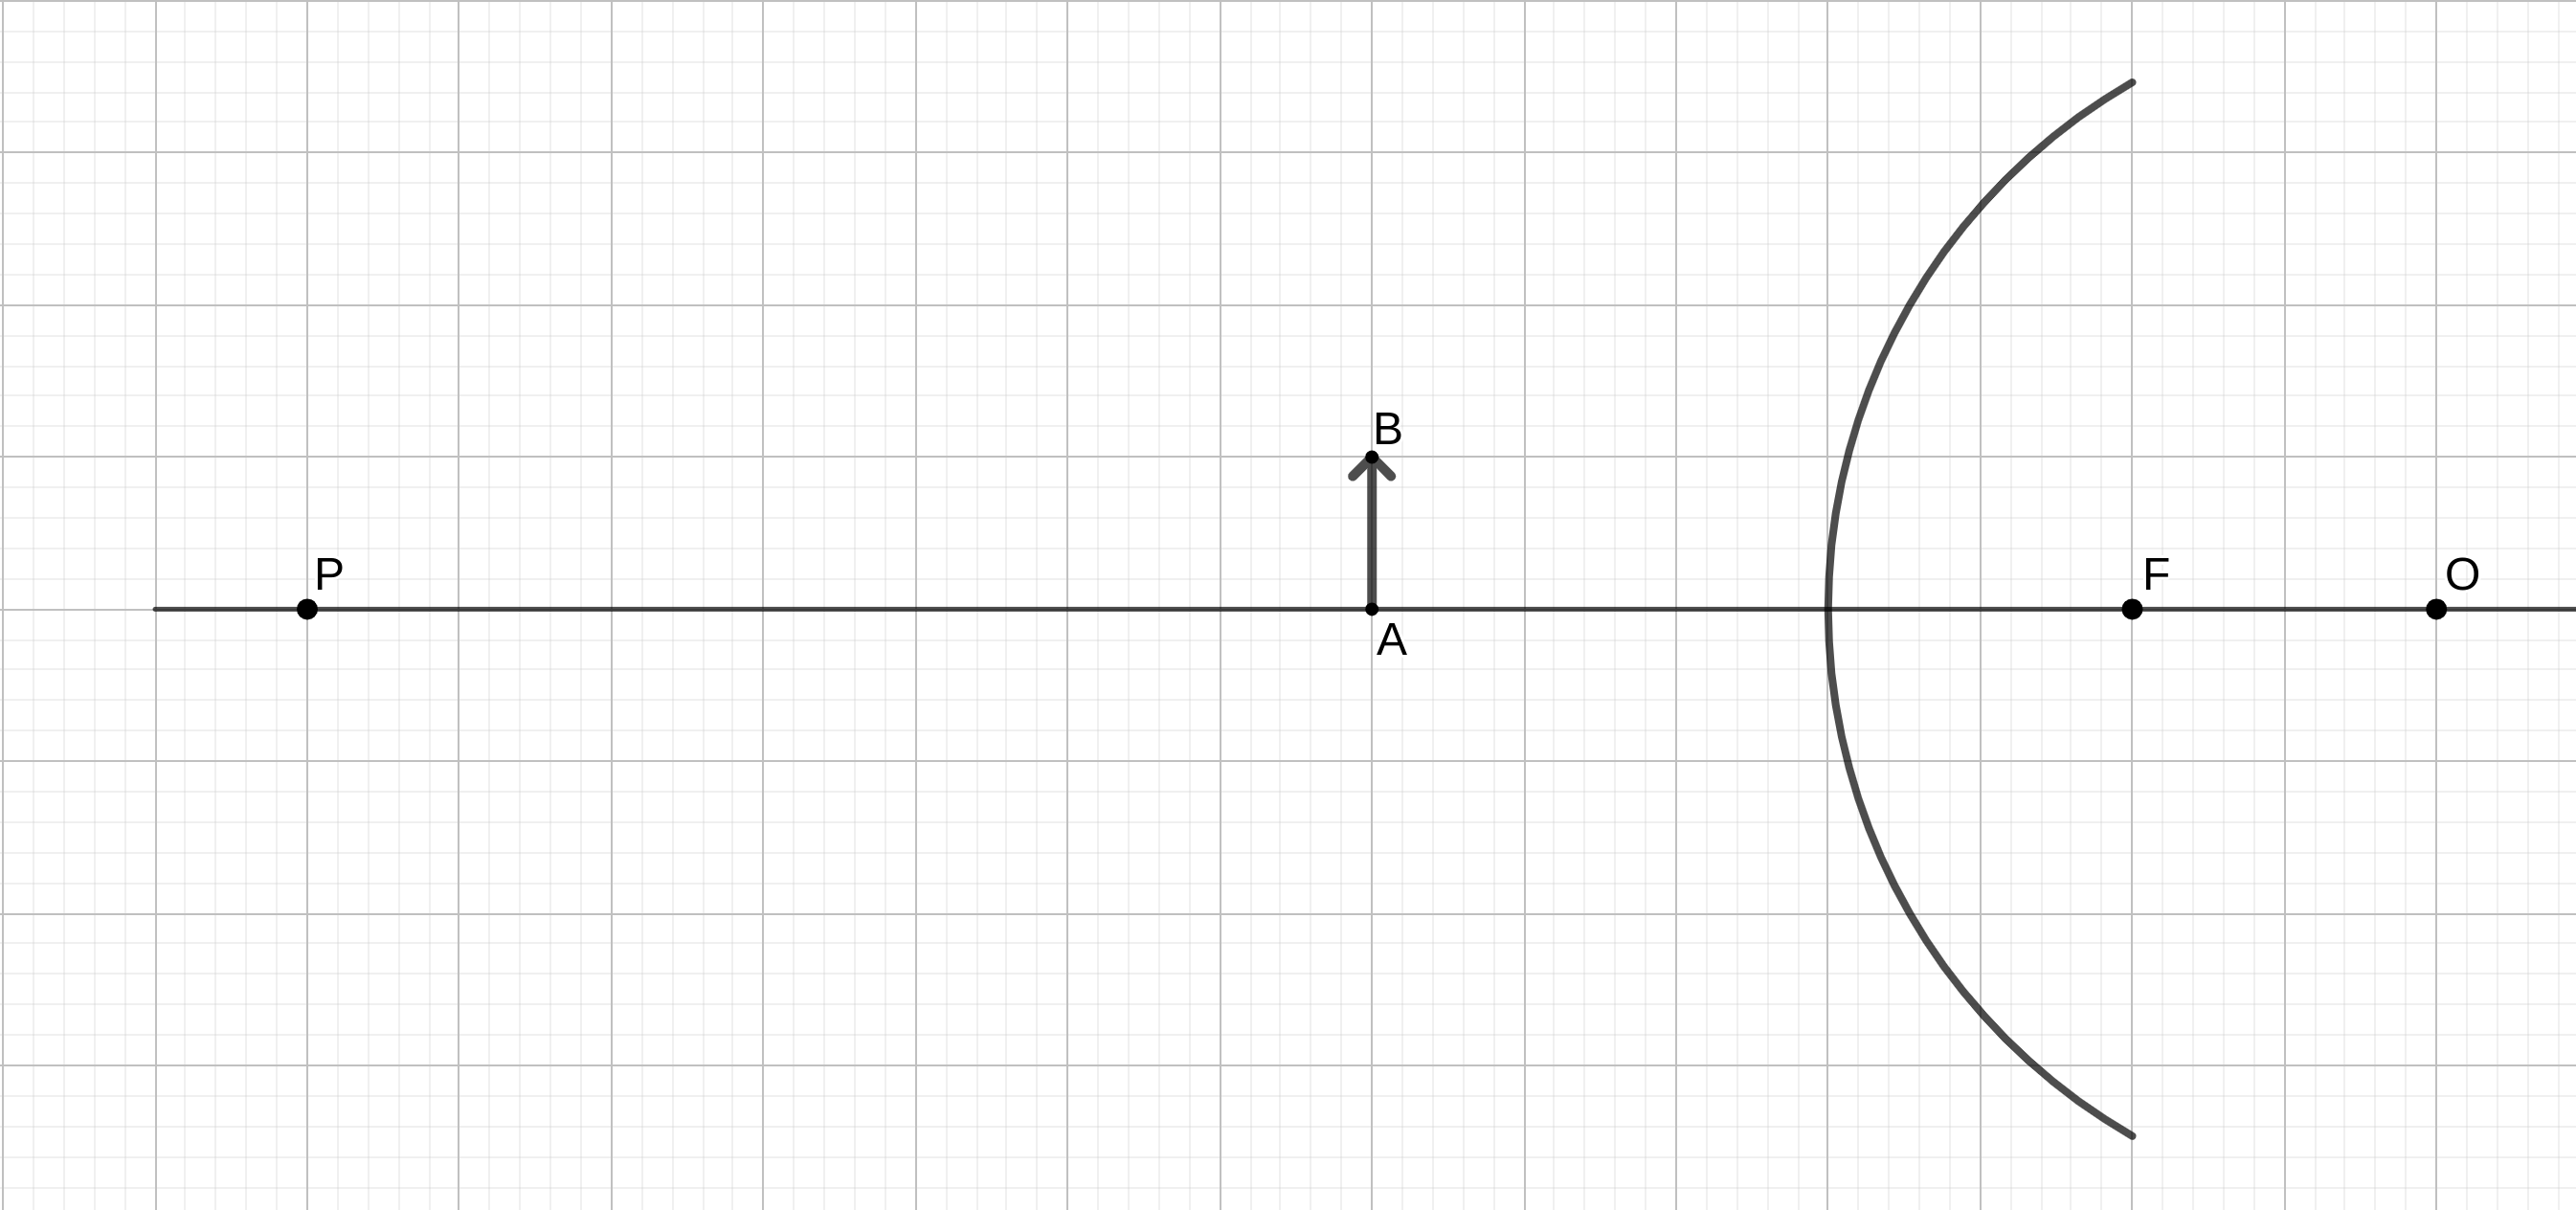
\includegraphics[width=0.75\linewidth]{2023-lahg-02-yl.png}
     \vspace{-20pt}
\end{figure}







\hint

\solu
\begin{figure}[h]
    \centering
    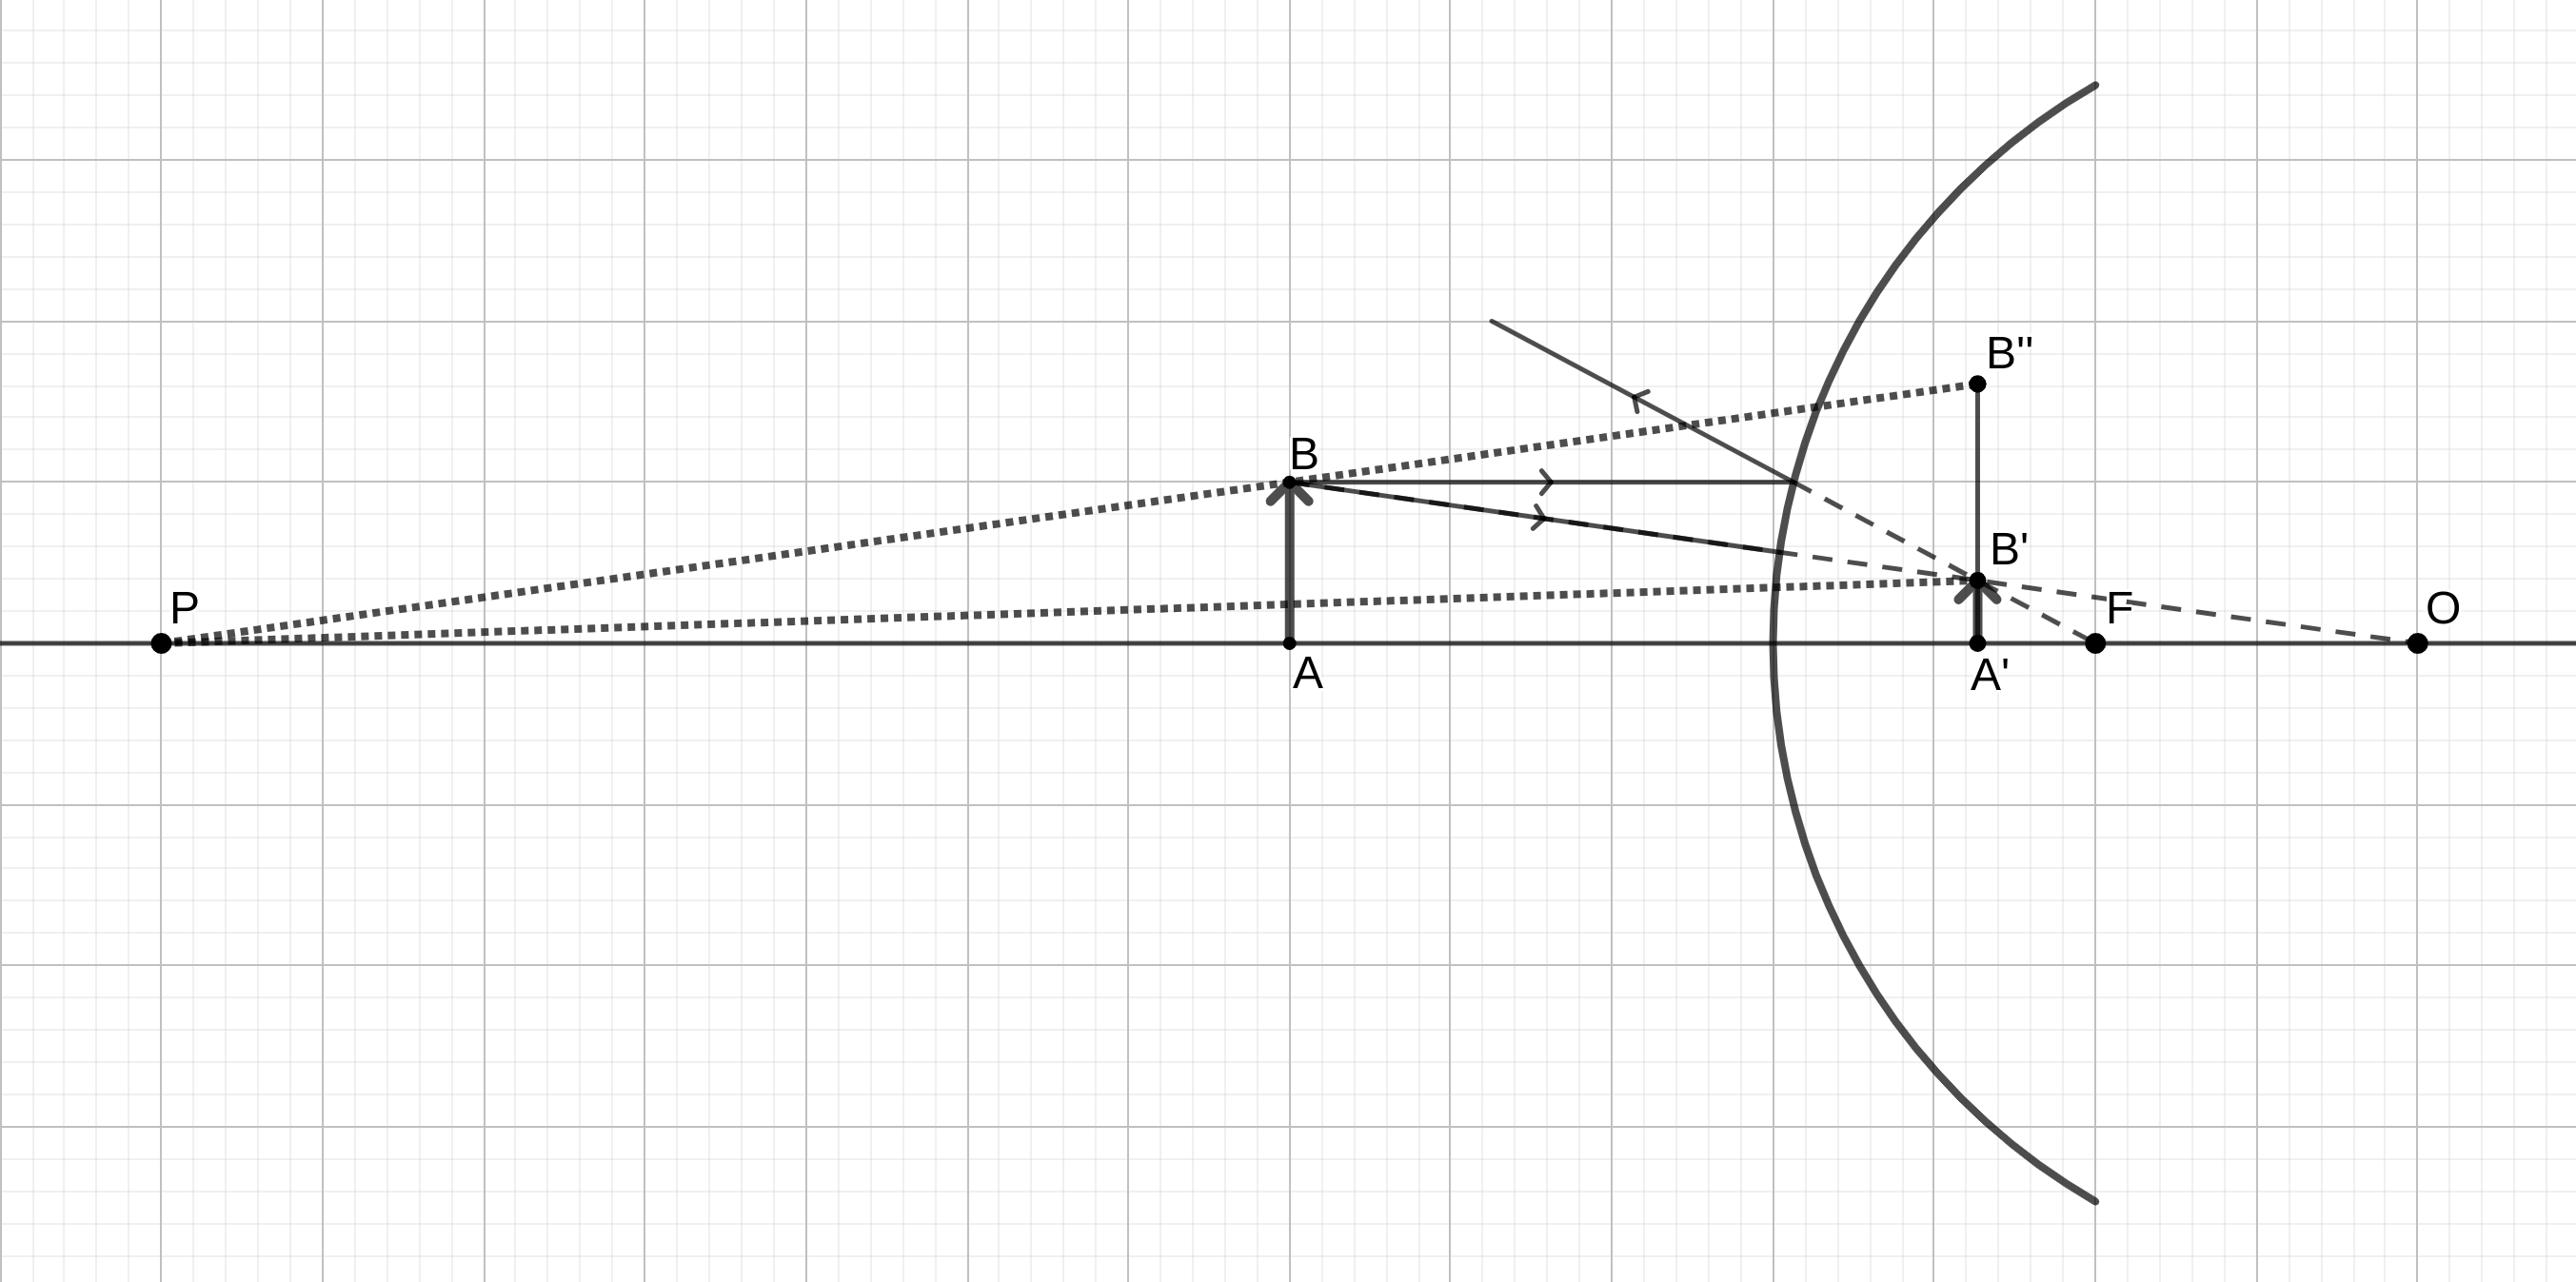
\includegraphics[width=\linewidth]{2023-lahg-02-sol.png}
\end{figure}

Ese paistab kumerpeeglis sama suur, kui suur paistaks selle kujutis ilma kumerpeeglita. Leiame kõigepealt eseme AB kujutise A'B', tõmmates ühe kiire otse läbi punkti O ja teise kiire kõigepealt paralleelselt optilise peateljega ja seejärel läbi fookuse F.

Selleks, et leida kui palju paistab kujutis A'B' väiksem esemest AB, peame lisaks füüsilisele suurusele arvestama ka kaugusega. Jooniselt näeme, et näivate suuruste suhe on sama, mis on lõikude A'B' ja A'B'' suhe. Jooniselt hindame, et A'B' pikkus on 2 ruutu ja A'B'' pikkus on 8 ruutu. Seega kumerpeeglis paistab ese 4 korda väiksem.
\probend